\documentclass[../../main.tex]{subfiles}

\begin{document}
\label{sec:abbildungen_graphen_intro}
\parpic[r]{
    \centering
    \begin{tikzpicture}[scale=.75]
    \draw[grayset] (-1.5,0) ellipse (0.7cm and 2cm);
    \draw[grayset] (1.5,0) ellipse (0.7cm and 2cm);

    \node (x1) at (-1.5,0.7) {$\bullet$};
    \node (x2) at (-1.5,-0.2) {$\bullet$};
    \node (x3) at (-1.5,-1.1) {$\bullet$};
    \node (y1) at (1.5,0.7) {$\bullet$};
    \node (y2) at (1.5,-0.2) {$\bullet$};
    \node (y3) at (1.5,-1.2) {$\bullet$};

    \draw[->] (x1) -- (y3);
    \draw[->] (x2) to[bend right] (y1);
    \draw[->] (x3) to[bend right] (y2);
\end{tikzpicture}%Also used by abbildungen/01einfuehrung
}

Zu Beginn des Kapitels haben wir bereits eine Möglichkeit gesehen, Funktionen graphisch darzustellen. Da eine Funktion eine Definitions- und eine Zielmenge hat, können wir diese beiden Mengen zeichnen und von jedem Argument einen Pfeil zu seinem Bild ziehen -- so wie in der Abbildung rechts. 

Diese Darstellung ist anschaulich, hat aber einen großen Nachteil: Wenn die Definitionsmenge viele oder sogar unendlich viele Elemente hat (z.B. wenn eine Funktion für alle natürlichen Zahlen, also \Natural, definiert ist), müssen wir selbst, wenn wir nur einen Ausschnitt zeichnen, sehr viele Pfeile zeichnen und es wird unübersichtlich.

Deshalb lernst du in diesem Abschnitt eine effektivere Methode kennen, die Koordinatensysteme verwendet. Ein Punkt im Koordinatensystem hat eine $x$- und eine $y$-Koordinate. Während die $x$-Koordinate angibt, wie weit rechts oder links er ist, sagt die $y$-Koordinate aus, wie weit oben oder unten der Punkt ist. Wo ein Punkt liegt, wird also durch zwei Informationen beschrieben.

\parpic[r]{
    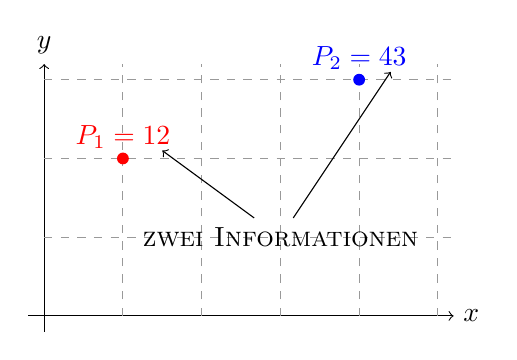
\begin{tikzpicture}
        \draw[->] (-0.2,0) -- (5.2,0) node[right] {$x$};
        \draw[->] (0,-0.2) -- (0,3.2) node[above] {$y$};
        \draw[dashed,black!40] (1,0) -- (1,3.2);
        \draw[dashed,black!40] (2,0) -- (2,3.2);
        \draw[dashed,black!40] (3,0) -- (3,3.2);
        \draw[dashed,black!40] (4,0) -- (4,3.2);
        \draw[dashed,black!40] (5,0) -- (5,3.2);
        \draw[dashed,black!40] (0,1) -- (5.2,1);
        \draw[dashed,black!40] (0,2) -- (5.2,2);
        \draw[dashed,black!40] (0,3) -- (5.2,3);
        \fill[red] (1,2) circle[radius=0.75mm] node[above] {$P_1=\coord{1}{2}$};
        \fill[blue] (4,3) circle[radius=0.75mm] node[above] {$P_2=\coord{4}{3}$};
        \node[align=center] (annotation) at (3,1) {\textsc{zwei Informationen}};
        \draw[->] (annotation) -- (4.4,3.1);
        \draw[->] (annotation) -- (1.5,2.1);
    \end{tikzpicture}
}

Jeder der Punkte $P_1$ und $P_2$, die du rechts siehst, benötigt zwei Informationen, um beschrieben zu werden. $P_1$ liegt bei $x$-Koordinate $1$ und $y$-Koordinate $2$. Würde eine dieser Informationen fehlen, wäre entweder nicht geklärt, wie weit rechts oder wie weit oben der Punkt liegt. Andersherum enthält die Position dieser Punkte natürlich auch genau diese zwei Informationen -- aus der Position von $P_2$ geht die $x$-Koordinate des Punktes ebenso wie die $y$-Koordinate hervor.

Wenn wir an die explizite Notation einer Zuordnungsvorschrift zurückdenken, dann hat jede Regel dort die Form $\text{Urbild}\mapsto\text{Bild}$. Sie enthält ebenfalls zwei Informationen -- erstens die Information über das Element der Definitionsmenge, das auf ein anderes abgebildet werden soll und zweitens die Information über das Bild dieses Elements.

Darauf aufbauend wollen wir die Koordinaten eines Punkts ab sofort nutzen, um eine Regel aus der Zuordnungsvorschrift darzustellen. Jeder Punkt soll für ein bestimmtes Element der Definitionsmenge darstellen, wohin es abgebildet wird.

\parpic[r]{
    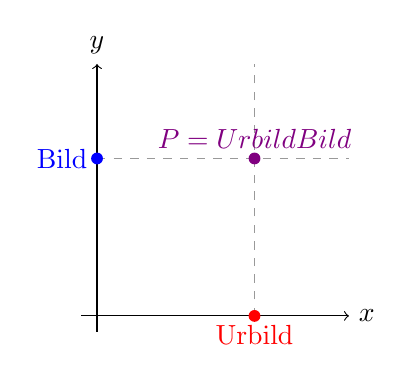
\begin{tikzpicture}
        \draw[->] (-0.2,0) -- (3.2,0) node[right] {$x$};
        \draw[->] (0,-0.2) -- (0,3.2) node[above] {$y$};
        \draw[dashed,black!40] (2,0) -- (2,3.2);
        \draw[dashed,black!40] (0,2) -- (3.2,2);
        %
        \fill[red] (2,0) circle[radius=0.75mm] node[below] {Urbild};
        \fill[blue] (0,2) circle[radius=0.75mm] node[left] {Bild};
        \fill[violet] (2,2) circle[radius=0.75mm] node[above] {$P=\coord{\text{Urbild}}{\text{Bild}}$};
    \end{tikzpicture}
}

Im Bild ist zu sehen, wie die Position des entsprechenden Punktes von Urbild und Bild abhängt: Wie weit rechts der Punkt ist, hängt davon ab, wie weit rechts das \emph{Argument} aus der Definitionsmenge auf der $x$-Achse liegt. Wie weit oben oder unten er ist, hängt davon ab, welches \emph{Bild} das Argument hat.

Die Punkte, die eingezeichnet werden sollen, bekommen die damit Koordinaten $P=\coord{\text{Urbild}}{\text{Bild}}$. Nach wie vor soll der erste Wert angeben, wie weit rechts der Punkt im Koordinatensystem liegt -- und der zweite Wert, wie weit oben.
Über jedem möglichen Argument für die Funktion ist also genau ein Punkt eingetragen, denn jedes Argument hat genau ein Bild (und auf der Höhe, die dem Bild entspricht, ist dieser Punkt eingetragen).

Da an den Achsen eines normalen Koordinatensystems Zahlen stehen, Funktionen aber beliebige Definitions- und Zielmengen haben können, ist erstmal unklar, wie Urbild-Bild-Paare angeben sollen, wie weit rechts oder links ein Punkt liegen muss. Die nächsten Abschnitte beschreiben, wie sich dieses Problem abhängig davon, welche Art von Definitionsmenge die Funktion hat, lösen lässt.

\subsection{Funktionsgraphen aus einzelnen Punkten}
\label{sec:abbildungen_graphen_diskret}

\parpic[r]{
    \begin{tikzpicture}[scale=0.8]
        \draw[grayset] (0,1.75) ellipse (3mm and 17.5mm);
        \draw[grayset] (1.8,0) ellipse (18mm and 3mm);
        \draw[->] (-0.2,0) -- (3.6,0);
        \draw[maincolor,<-] (0.1,2.5) to[bend left] (1,2.8) node[maincolor,right] {\scriptsize Zielmenge};
        \draw[->] (0,-0.2) -- (0,3.5);
        \draw[maincolor,<-] (2.5,0.1) to[bend right] (2,1) node[maincolor,above] {\scriptsize Definitionsmenge};
        \fill (0,1) circle[radius=0.1];
        \fill (0,2) circle[radius=0.1];
        \fill (0,3) circle[radius=0.1];
        \fill (1,0) circle[radius=0.1];
        \fill (2,0) circle[radius=0.1];
        \fill (3,0) circle[radius=0.1];
    \end{tikzpicture}
}

Um Funktionen im Koordinatensystem zu beschreiben, ist es notwendig, die Definitions- und Zielmenge im Koordinatensystem zu repräsentieren. Dafür nutzt man die beiden Achsen des Koordinatensystems: Die Definitionsmenge liegt quer, sodass die einzelnen Elemente davon auf der $x$-Achse untergebracht werden können. Die Zielmenge wird so eingezeichnet, dass sich ihre Elemente als Punkte auf der $y$-Achse einzeichnen lassen.

Es spielt erstmal keine Rolle, in welcher Reihenfolge die Elemente eingezeichnet werden. Wichtig ist nur, dass sie alle auf der entsprechenden Koordinatenachse liegen. Mit diesem Schritt bereiten wir das Koordinatensystem vor, um im zweiten Schritt die Zuordnungsvorschrift einzeichnen zu können.

\begin{example}{}
    \parpic[r]{
        \begin{tikzpicture}[scale=0.7]
            \draw[grayset] (0,1.75) ellipse (3mm and 1.75cm);
            \draw[grayset] (2.5,0) ellipse (25mm and 3mm);
            %
            \draw[->] (-0.2,0) -- (5.5,0);
            \draw[->] (0,-0.2) -- (0,3.8);
            %
            \node[maincolor] (D) at (3,1) {\scriptsize\textsc{Grundfarben}};
            \node[maincolor] (B) at (3,3) {\scriptsize\textsc{Mischfarben}};
            \draw[maincolor,->] (D) -- (3.5,0.1);
            \draw[maincolor,->] (B.west) to[bend right] (0.1,2.3);
            %
            \fill[yellow!70!black] (0,1) circle[radius=0.1] node[black, left] {\scriptsize gelb};
            \fill[orange] (0,2) circle[radius=0.1] node[black, left] {\scriptsize orange};
            \fill[green!70!black] (0,3) circle[radius=0.1] node[black, left] {\scriptsize grün};
            %
            \fill[yellow!70!black] (1.5,0) circle[radius=0.1] node[black, below] {\scriptsize gelb};
            \fill[red] (3,0) circle[radius=0.1] node[black, below] {\scriptsize rot};
            \fill[blue] (4.5,0) circle[radius=0.1] node[black, below] {\scriptsize blau};
        \end{tikzpicture}
    }
    %\picskip{7}
    Nachdem das Koordinatensystem vorbereitet wurde, um die Funktion \textsc{MitGelbMischen} im Koordinatensystem darzustellen, sieht es wie rechts abgebildet aus: Die Definitionsmenge von \textsc{MitGelbMischen} ist die Menge \textsc{Grundfarben}. Diese ist auf der $x$-Achse eingezeichnet.
    
    Die Zielmenge (die Menge \textsc{Mischfarben}) wird über die $y$-Achse gelegt. Damit kann jede Mischfarbe einen Punkt auf der $y$-Achse erhalten.
\end{example}

Jetzt ist es möglich, für jede Zuordnungsregel der Form $\text{Urbild}\mapsto\text{Bild}$ den Punkt $\coord{\text{Urbild}}{\text{Bild}}$ einzuzeichnen. Dafür wird der Punkt in gerader Linie über dem Urbild eingezeichnet. Das Urbild wurde im vorherigen Schritt an einer Stelle auf der $x$-Achse platziert. Die Höhe des Punktes entspricht der Höhe, an der auf der $y$-Achse das Bildelement eingetragen wurde. Zeichnet man also vom Urbild eine Linie nach oben und vom Bild eine Linie nach rechts, dann stellt der Schnittpunkt die Zuordnungsregel für diese beiden Elemente dar.

\begin{example}{}
    \parpic[r]{
        \begin{tikzpicture}[scale=0.8]
            \draw[->] (-0.2,0) -- (5.1,0) node[right,text width=2cm] {\scriptsize \textsc{Grundfarben}};
            \draw[->] (0,-0.2) -- (0,3.5) node[above] {\scriptsize \textsc{Mischfarben}};
            %
            \draw[dashed] (1.5,0) -- (1.5,1);
            \draw[dashed] (3,0) -- (3,2);
            \draw[dashed] (4.5,0) -- (4.5,3);
            \draw[dashed] (0,1) -- (1.5,1);
            \draw[dashed] (0,2) -- (3,2);
            \draw[dashed] (0,3) -- (4.5,3);
            %
            \fill[yellow!70!black] (0,1) circle[radius=0.1] node[black, left] {\scriptsize gelb};
            \fill[orange] (0,2) circle[radius=0.1] node[black, left] {\scriptsize orange};
            \fill[green!70!black] (0,3) circle[radius=0.1] node[black, left] {\scriptsize grün};
            %
            \fill[yellow!70!black] (1.5,0) circle[radius=0.1] node[black, below] {\scriptsize gelb};
            \fill[red] (3,0) circle[radius=0.1] node[black, below] {\scriptsize rot};
            \fill[blue] (4.5,0) circle[radius=0.1] node[black, below] {\scriptsize blau};
            %
            \fill (1.5,1) circle[radius=0.1] node[black, above] {\scriptsize $\text{gelb}\mapsto\text{gelb}$};
            \fill (3,2) circle[radius=0.1] node[black, above] {\scriptsize $\text{rot}\mapsto\text{orange}$};
            \fill (4.5,3) circle[radius=0.1] node[black, above] {\scriptsize $\text{blau}\mapsto\text{grün}$};
        \end{tikzpicture}
    }
    
    Im nebenstehenden Bild wurden die Zuordnungsregeln durch die drei eingezeichneten schwarzen Punkte dargestellt. Der Punkt mit der Beschriftung $\text{blau}\mapsto\text{grün}$ liegt in gerader Linie über dem Urbild (blau) und in gerader Linie neben dem Bild (grün). So ist es möglich, am Punkt abzulesen, welche Regel er darstellt, auch wenn die Beschriftung nicht vorhanden wäre.
\end{example}

Durch das ungeordnete Eintragen der Definitions- und Zielmenge auf den Achsen hat man zunächst relativ wenig aus dem Koordinatensystem herausgeholt. Die Darstellung ist zunächst überhaupt nicht übersichtlicher. Das liegt daran, dass wir bisher nicht genutzt haben, dass sich bei Koordinatensystemen normalerweise eine Ordnung auf den Achsen befindet: Nach rechts bzw. oben werden die Werte immer größer.

Manche Definitions- und Zielmengen lassen es zu, dass wir ihre Elemente sinnvoll ordnen, etwa alphabetisch oder -- wenn es sich um Zahlen handelt -- nach der Größe.

Auf diese Weise kann es möglich sein, durch die Anordnung der Punkte durch kurzes Hinsehen sofort Informationen darüber zu erhalten, wie eine Zuordnungsvorschrift aufgebaut ist. 

\parpic[r]{
    \begin{tikzpicture}[scale=0.7]
        \begin{axis}[defgrid, domain=-2:2, y=1cm, x=1cm, xmin=0, xmax=4, ymin=0,ymax=4,xtick={1,...,4}, ytick={1,...,4}]
        \end{axis}
        \if 0
        \draw[->] (-0.2,0) -- (5.6,0) node[right] {$x$};
        \draw[->] (0,-0.2) -- (0,4.2) node[above] {$f(x)$};
        \foreach\y in {1,...,4}{
            \fill[blue] (0,\y) circle[radius=0.1] node[black, left] {$\y$};
        }
        \foreach\x in {0,...,5}{
            \fill[red] (\x,0) circle[radius=0.1] node[black, below] {$\x$};
        }
        \fi
    \end{tikzpicture}
}

Gerade wenn man es mit Funktionen zu tun hat, die nur mit Zahlen arbeiten, kann man einfach das gewohnte Koordinatensystem verwenden und für jede Zahl, die tatsächlich in der Definitionsmenge ist, einen Punkt auf der $x$-Achse eintragen (bzw. auf der $y$-Achse für Zahlen in der Zielmenge).

Rechts siehst du ein Koordinatensystem, das sich direkt eignet, um Funktionen darzustellen, die Zahlen zu Zahlen zuordnen. Weil ohnehin jede Zahl einen Platz auf der $x$-Achse oder $y$-Achse hat, muss dort nicht noch zusätzlich eine Menge eingezeichnet werden.

\begin{example}[ex:graph-for-n]{}
    \parpic[r]{
        \begin{tikzpicture}
            \begin{axis}[defgrid, domain=-2:2, y=1cm, x=1cm, xmin=0, xmax=4, ymin=0,ymax=4,xtick={1,...,4}, ytick={1,...,4}]
                \draw[dashed, very thick] (0,1) -- (0,0);
                \draw[dashed, very thick] (0,2) -- (1,2) -- (1,0);
                \draw[dashed, very thick] (0,3) -- (2,3) -- (2,0);
                \draw[dashed, very thick] (0,4) -- (3,4) -- (3,0);
                \addplot[mark=*, only marks, fill=violet] coordinates {(0,1)};
                \addplot[mark=*, only marks, fill=violet] coordinates {(1,2)};
                \addplot[mark=*, only marks, fill=violet] coordinates {(2,3)};
                \addplot[mark=*, only marks, fill=violet] coordinates {(3,4)};
            \end{axis}
        \end{tikzpicture}
    }

    Im abgebildeten Koordinatensystem ist die Funktion $f\colon\Natural\rightarrow\Natural$ zu sehen, die jeder Zahl ihren Nachfolger zuordnet. $f$ ist also durch die Berechnungsvorschrift $f(x)=x+1$ definiert.
    
    Die lilafarbenen Punkte, die zum Darstellen der Zuordnungsvorschrift eingezeichnet wurden, sind in einem bestimtmen Muster angeordnet: Sie bilden eine nach oben führende Gerade. Diese Gerade würde natürlich auch nach rechts weitergehen, wenn ein größeres Koordinatensystem zur Verfügung stehen würde.
    
    \parpic[r]{1}
    Allein durch das kurze Betrachten des Bildes weißt du sofort etwas über die Zuordnungsvorschrift (zum Beispiel, dass du größere Zahlen als Bilder du erhältst, je größer du das Argument wählst).
\end{example}

In den meisten mathematischen Anwendungen arbeitet man mit Funktionen, die unendlich viele verschiedene Argumente erhalten können, also eine unendliche Definitionsmenge haben. Das ist zum Beispiel bei Funktionen, deren Definitionsmenge die natürlichen Zahlen sind, der Fall. Deswegen stellen wir meistens nur einen bestimmten Ausschnitt der Zuordnungsvorschrift dar.

In Beispiel \ref{ex:graph-for-n} endete die $y$-Achse beispielsweise bei der $4$. Das heißt, dass in diesem Koordinatensystem einfach alle Zuordnungsregeln für Zahlen, deren Bilder größer als $4$ sind, nicht mehr dargestellt werden. Das ist grundsätzlich kein Problem -- sondern sogar notwendig, da es ja nicht möglich ist, unendlich viele Punkte einzuzeichnen. Wenn man von einer Funktion, die für alle natürliche Zahlen definiert ist, nur einen ausgewählten Bereich zeichnet, hat man automatisch wieder eine kleine, endliche Anzahl an Punkten übrig, die man einzeichnen muss.

Die Gesamtheit aller Punkte, die man zum Darstellen der Zuordnungsvorschrift ins Koordinatensystem einzeichnet, nennt man den \textbf{Graphen} der Funktion. Im letzten Beispiel bestand der Graph von $f$ beispielsweise aus allen lilafarbenen Punkten.

\begin{definition}{Graph einer Funktion}
        Für eine Funktion $f\colon U\rightarrow V$ mit $U,V\subseteq \Real$ ist der \textbf{Graph} von $f$ die Menge aller Punkte $\coord{x}{y}$ im Koordinatensystem, für die $f(x)=y$ gilt. Der Graph von $f$ ist also die Menge $\{\coord{x}{y} \mid f(x)=y\}$.
\end{definition}

\subsection{Funktionsgraphen aus unendlich vielen Punkten}
\label{sec:abbildungen_graphen_stetig}

Obwohl es nicht möglich ist, Funktionen mit unendlicher Definitionsmenge vollständig graphisch darzustellen, gibt es eine gute Möglichkeit, sie trotzdem sinnvoll aufzuzeichnen. Im letzten Abschnitt hast du gesehen, dass du nur eine kleine Anzahl an Punkten zeichnen musst, wenn du nur ein Intervall aus der Definitionsmenge darstellst.

Eine Funktion $f\colon\Natural\rightarrow\Natural$ lässt sich beispielsweise zeichnen, indem du die Definitionsmenge nur bis zur Zahl $5$ (oder einer beliebigen anderen Zahl) darstellst. Dann besteht der Teil des Funktionsgraphen, den du zeichnen musst, nur aus fünf Punkten. Dieser Trick funktioniert nicht bei Definitionsmengen, bei denen in beliebig kleinen Bereichen schon unendlich viele Elemente auftauchen. Das ist zum Beispiel bei den reellen Zahlen der Fall, weil sich (fast) lückenlos auf jedem Punkt der $x$-Achse eine reelle Zahl befindet.

\if 0
\begin{advanced}{Dichte Mengen}
    Eine Menge ist dicht, wenn sich zwischen zwei beliebigen Zahlen aus der Menge immer noch eine weitere Zahl finden lässt, die zwischen den beiden Zahlen liegt.
    
    \begin{definition}{Dichte Menge}
        Eine Menge $M$ heißt \textbf{dicht}, wenn für beliebige $m,m'\in M$ ein $x\in M$ existiert mit $m<x<m'$.
    \end{definition}
    
    \begin{example}{}
        Die Menge $\Rational$ ist dicht. Wählt man zum Beispiel die Zahlen $0$ und $1$, so liegt die Zahl $\frac{1}{2}$ zwischen diesen Zahlen. Egal wie klein man den Abstand zweier Zahlen wählt -- selbst, wenn man $0.0001$ und $0.0002$ wählt -- es gibt immer eine rationale Zahl zwischen den beiden Zahlen.
    \end{example}
\end{advanced}
\fi

Warum sind solche Definitionsmengen nun ein Problem? Wenn du einen Graphen für eine Funktion mit einer Definitionsmenge wie den reellen Zahlen zeichnen möchtest, kannst du zwar links und rechts die Definitionsmenge abschneiden, indem du die Zeichnung dort aufhören lässt. Das Problem ist, dass trotzdem immer unendlich viele mögliche Argumente in deinem Bild auftauchen -- egal, wie weit du den Bereich einschränkst.

Nun sehen wir uns an, wie man das Zeichnen von unendlich vielen Punkten auch für solche Funktionen vermeiden kann.

\begin{example}{}
    \begin{minipage}{\textwidth}
        Der Graph der Funktion $f\colon\Real\rightarrow\Real$ mit $f(x)=1$ enthält die Punkte $\coord{0}{1}, \coord{1}{1}, \coord{2}{1}$ und $\coord{3}{1}$. Diese Punkte gehören in jedem Fall zum Graphen von $f$. Sie können also sofort eingezeichnet werden. Man erhält eine Darstellung wie links.
        
        Anschließend fehlen weiterhin alle Punkte zwischen den eingezeichneten. Man kann also fortfahren, indem man auch einige davon einzeichnet -- und nächsten Schritt noch mehr. Schrittweise kommt man so zum mittleren bzw. rechten Bild.
        
        Macht man auf diese Weise immer weiter, dann haben die Punkte irgendwann keinen sichtbaren Abstand mehr und bilden letztlich einfach eine durchgezogene Linie.
        
        \begin{multicols}{3}
            \centering
            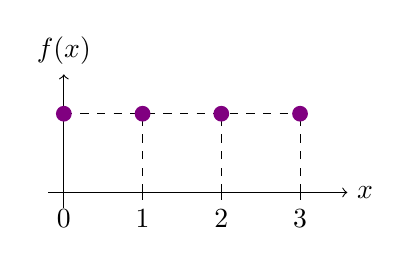
\begin{tikzpicture}
                \draw[->] (-0.2,0) -- (3.6,0) node[right] {$x$};
                \draw[->] (0,-0.2) -- (0,1.5) node[above] {$f(x)$};
                
                \draw[dashed] (0,1) -- (3,1);
                \foreach \x in {0,1,...,3}{
                    \draw (\x,0.1) -- (\x,-0.1) node[black, below] {$\x$};
                    \draw[dashed] (\x,0) -- (\x,1);
                    \fill[violet] (\x,1) circle[radius=0.1];
                }
            \end{tikzpicture}
            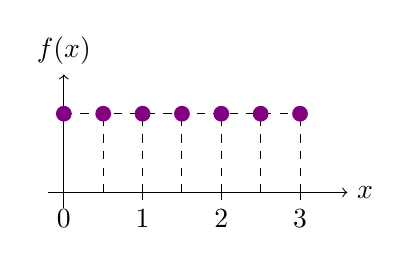
\begin{tikzpicture}
                \draw[->] (-0.2,0) -- (3.6,0) node[right] {$x$};
                \draw[->] (0,-0.2) -- (0,1.5) node[above] {$f(x)$};
                
                \draw[dashed] (0,1) -- (3,1);
                \foreach \x in {0,0.5,...,3}{
                    \draw[dashed] (\x,0) -- (\x,1);
                    \fill[violet] (\x,1) circle[radius=0.1];
                }
                \foreach \x in {0,1,...,3}{
                    \draw (\x,0.1) -- (\x,-0.1) node[black, below] {$\x$};
                }
            \end{tikzpicture}
            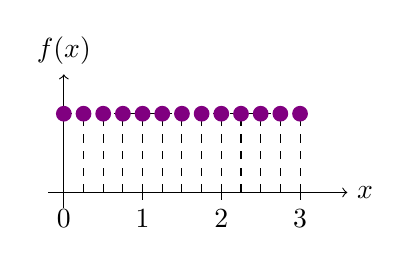
\begin{tikzpicture}
                \draw[->] (-0.2,0) -- (3.6,0) node[right] {$x$};
                \draw[->] (0,-0.2) -- (0,1.5) node[above] {$f(x)$};
                
                \draw[dashed] (0,1) -- (3,1);
                \foreach \x in {0,0.25,...,3}{
                    \draw[dashed] (\x,0) -- (\x,1);
                    \fill[violet] (\x,1) circle[radius=0.1];
                }
                \foreach \x in {0,1,...,3}{
                    \draw (\x,0.1) -- (\x,-0.1) node[black, below] {$\x$};
                }
            \end{tikzpicture}
        \end{multicols}
    \end{minipage}
\end{example}

Um den Graphen auch bei dichten Definitionsmengen zu zeichnen, kann man zunächst anfangen, indem man einige beliebige Punkte, die ins Bild passen, einzeichnet. Diese Punkte gehören auf jeden Fall zum Graphen. Zeichnet man nun einige weitere Punkte dazwischen, dann entwickelt sich der Graph wie im letzten Beispiel.

Aus einzelnen Punkten wird eine zusammenhängende Linie, weil es keinen freien Platz zwischen den einzelnen Punkten mehr gibt. Sobald du das vorher weißt, kannst du auch einfach direkt die Linie zeichnen, die du am Ende bekommen wirst. Es hilft aber dennoch, zunächst einzelne Punkte einzuzeichnen, damit du siehst, wie der Graph am Ende aussehen wird und wo du die Linie zeichnen musst.

\begin{example}{}
    \parpic[r]{
        \begin{tikzpicture}
            \draw[->] (-0.2,0) -- (3.6,0) node[right] {$x$};
            \draw[->] (0,-0.2) -- (0,1.5) node[above] {$f(x)$};
            \foreach \x in {0,...,3}{
                \draw (\x,0.1) -- (\x,-0.1) node[black, below] {$\x$};
                \draw[dashed] (\x,0) -- (\x,1);
            }
            \draw[violet] (0,1) -- (3.3,1);
        \end{tikzpicture}
    }
    
    \picskip{7}
    Die Funktion aus dem letzten Beispiel hat den rechts dargestellten Graphen, der direkt als eine Linie gezeichnet wurde. Man kann es sich sparen, vorher einzelne Punkte einzuzeichnen, weil am Ende sowieso alle Punkte zu einer einzelnen Linie verschmelzen, wenn wir die reellen Zahlen als Definitionsmenge verwenden.
    
    Die eingezeichneten gestrichelten Linien dienen als Beispiele, bei welchen Argumenten du anfangen kannst, einzelne Punkte auf dem Graphen zu finden, um zu sehen, wo die Linie entlangführt, die am Ende gezeichnet werden muss. Man hätte genauso gut an irgendeiner anderen Stelle ein Bild zu einem Argument berechnen und eine Linie zeichnen können. Grundsätzlich lässt man die gestrichelten Linien später einfach weg -- sie können aber dabei helfen, eine solche graphische Darstellung zu zeichnen.
\end{example}

Mithilfe des Koordinatensystems können wir nun Eigenschaften von Funktionen \emph{sehen}. Für Funktionen, die nicht so einfach sind, kann es später sehr hilfreich sein, sich mithilfe von Koordinatensystemen Informationen zu beschaffen, um sie besser zu verstehen.

Wir sind außerdem in der Lage, die Zuordnungsregeln direkt im Koordinatensystem abzulesen. Dafür starten wir auf der $x$-Achse bei einem Wert, dessen Bild wir suchen. Von diesem Wert aus gehen wir in gerader Linie nach oben, bis wir den Graphen treffen. Auf der Höhe, auf der wir auf den Graphen treffen, befindet sich auf der $y$-Achse auch das Bild, das wir suchen.

Auf ähnliche Weise können wir vorgehen, wenn wir die Urbilder zu einem Element der Zielmenge suchen -- wir fangen dann bei der $y$-Achse an und suchen den Graphen auf einer geraden Linie nach links oder rechts. Allerdings muss man dann damit rechnen, dass man mehrere oder gar kein passendes Urbild findet (z.B. wenn die Funktion das gewählte Bild keinem Element der Definitionsmenge zugeordnet hat).

\begin{example}{}
    \parpic[r]{
        \tikz{
            \begin{axis}[defgrid, domain=0:4, y=1cm, x=1cm, xmin=0, xmax=4, ymin=0,ymax=4,xtick={1,...,4}, ytick={1,...,4}]
                \draw[dashed, very thick, ->] (2,0) -- (2,3) -- (0,3);
                \addplot[color=violet] expression{x+1};
                \addplot[mark=*, only marks, fill=violet] coordinates {(2,3)};
            \end{axis}
        }
    }

    Am rechts abgebildeten Funktionsgraphen können die Bilder von beliebigen Elementen der Definitionsmenge abgelesen werden. Um beispielsweise abzulesen, welcher Zahl das Argument $2$ zugeordnet wird, beginnst du dort, wo die Zahl $2$ auf der $x$-Achse eingetragen ist und schaust dann auf einer geraden Linie nach oben, wo du den Graphen triffst.
    
    \picskip{2}
    In diesem Fall triffst du den Graphen beim eingezeichneten lilafarbenen Punkt. Um nun herauszufinden, welchem Element der Zielmenge der getroffene Punkt entspricht, verfolgst du vom eingezeichneten Punkt eine gerade Linie nach links, bis du die $y$-Achse triffst. Vom lila eingezeichneten Punkt kommst du zur $3$. Dies ist das Bild, das wir gesucht haben. Es gilt also $f(2)=3$.
\end{example}

\begin{nutshell}{Funktionen in Koordinatensystemen darstellen}
    \parpic[r]{
        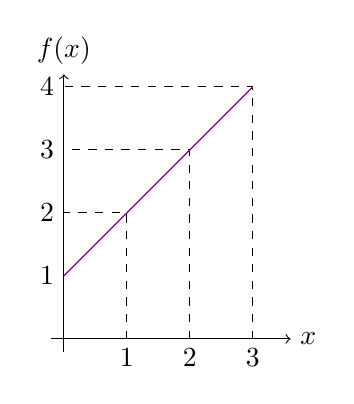
\begin{tikzpicture}[scale=0.8]
            \draw[->] (-0.2,0) -- (3.6,0) node[right] {$x$};
            \draw[->] (0,-0.2) -- (0,4.2) node[above] {$f(x)$};
            %
            \draw[dashed] (0,0) -- (0,1) node[left]{$1$};
            \draw[dashed] (1,0) node[below]{$1$} -- (1,2) -- (0,2) node[left]{$2$};
            \draw[dashed] (2,0) node[below]{$2$} -- (2,3) -- (0,3) node[left]{$3$};
            \draw[dashed] (3,0) node[below]{$3$} -- (3,4) -- (0,4) node[left]{$4$};
            %
            \draw[violet] (0,1) -- (3,4);
        \end{tikzpicture}
    }
    
    Die Darstellung von Funktionen mit Mengendiagrammen ist bei großen Definitionsmengen sehr unpraktisch und die Pfeile stellen die Zuordnungsvorschrift nicht übersichtlich dar.
    
    Deswegen stellt man Funktionen normalerweise im Koordinatensystem dar, indem man einen \textbf{Funktionsgraphen} einzeichnet. Dafür stellt die $x$-Achse die Elemente der Definitionsmenge und die $y$-Achse die Elemente der Zielmenge dar. Über jedem $x$-Wert wird ein Punkt auf der Höhe seines Bildes eingezeichnet. 
    
    \picskip{1}
    Ist die Definitionsmenge lückenlos, dann verbindet man die eingezeichneten Punkte zu einer durchgehenden Linie, um den Graphen der Funktion zu erhalten.
\end{nutshell}

\end{document}